%!Mode:: "TeX:UTF-8"
\documentclass[a4paper,11pt,UTF8]{ctexart}

\usepackage{indentfirst} %缩进
\usepackage{xeCJK}    %使用系统字体
\usepackage{fancyhdr} %自定义页眉页脚
\pagestyle{empty}                   %不设置页眉页脚
\usepackage{amsmath, amsthm, amssymb, amsfonts} %数学公式
\usepackage[a4paper,left=3cm,right=3cm,top=3cm,bottom=3cm]{geometry}
%\usepackage[tmargin=1in,bmargin=1in,lmargin=1.25in,rmargin=1.25in]{geometry}.
\usepackage{booktabs} %插入表格
\usepackage[section]{placeins} %避免浮动
\usepackage{listings} %插入代码
\usepackage{ctex}     %中文宏包
\usepackage[svgnames, table]{xcolor} %彩色表格
\usepackage{algorithm}          %伪代码
\usepackage{algorithmicx}
\usepackage{algpseudocode}
\usepackage{algorithm,algpseudocode,float}
\usepackage{lipsum}
\usepackage{enumitem}           %调整列举环境
\usepackage{url}
\usepackage{fontspec,xunicode}
\defaultfontfeatures{Mapping=tex-text} %如果没有它,会有一些 tex 特殊字符无法正常使用,比如连字符。

\usepackage{graphicx}
\graphicspath{{imgs/}}

%%%%%%%%%%%%%%%%%%%%%%%%%%%%%%%%%%%%%%%%%%%%%%%%%%%%%%%%%%%%%%%%
% 缩进及行间距
%%%%%%%%%%%%%%%%%%%%%%%%%%%%%%%%%%%%%%%%%%%%%%%%%%%%%%%%%%%%%%%%
\setlength{\parindent}{22pt} %重新定义缩进长度
\setlength{\baselineskip}{20pt}  %定义行间距
%\renewcommand{\baselinestretch}{1.1} %定义行间距

%%%%%%%%%%%%%%%%%%%%%%%%%%%%%%%%%%%%%%%%%%%%%%%%%%%%%%%%%%%%%%%%
% 列表设置
%%%%%%%%%%%%%%%%%%%%%%%%%%%%%%%%%%%%%%%%%%%%%%%%%%%%%%%%%%%%%%%%
\setenumerate{fullwidth,itemindent=\parindent,listparindent=\parindent,itemsep=0ex,partopsep=0pt,parsep=0ex}
\setenumerate[2]{label=\alph*),leftmargin=1.5em}  %二级item设置
\setitemize{itemindent=38pt,leftmargin=0pt,itemsep=-0.4ex,listparindent=26pt,partopsep=0pt,parsep=0.5ex,topsep=-0.25ex}
\setdescription{itemindent=38pt,leftmargin=0pt,itemsep=-0.4ex,listparindent=26pt,partopsep=0pt,parsep=0.5ex,topsep=-0.25ex}

%%%%%%%%%%%%%%%%%%%%%%%%%%%%%%%%%%%%%%%%%%%%%%%%%%%%%%%%%%%%%%%%
% 图的标题行间距设置
%%%%%%%%%%%%%%%%%%%%%%%%%%%%%%%%%%%%%%%%%%%%%%%%%%%%%%%%%%%%%%%%
\newcommand{\bottomcaption}{%
\setlength{\abovecaptionskip}{6pt}%
\setlength{\belowcaptionskip}{6pt}%
\caption}


%%%%%%%%%%%%%%%%%%%%%%%%%%%%%%%%%%%%%%%%%%%%%%%%%%%%%%%%%%%%%%%%
% 字体定义
%%%%%%%%%%%%%%%%%%%%%%%%%%%%%%%%%%%%%%%%%%%%%%%%%%%%%%%%%%%%%%%%
\setmainfont{Times New Roman}  %默认英文字体.serif是有衬线字体sans serif无衬线字体
\setmonofont{Consolas}
\setCJKmainfont[ItalicFont={楷体}, BoldFont={黑体}]{宋体}%衬线字体 缺省中文字体为
\setCJKsansfont{黑体}
\punctstyle{hangmobanjiao}
%-----------------------xeCJK下设置中文字体------------------------------%
\setCJKfamilyfont{song}{SimSun}                             %宋体 song
\newcommand{\song}{\CJKfamily{song}}
\setCJKfamilyfont{fs}{FangSong}                      %仿宋  fs
\newcommand{\fs}{\CJKfamily{fs}}
\setCJKfamilyfont{ktgb}{KaiTi}                      %楷体2312 ktgb
\newcommand{\ktgb}{\CJKfamily{ktgb}}
\setCJKfamilyfont{yh}{Microsoft YaHei}                    %微软雅黑 yh
\newcommand{\yh}{\CJKfamily{yh}}
\setCJKfamilyfont{hei}{SimHei}                              %黑体  hei
\newcommand{\hei}{\CJKfamily{hei}}
\setCJKfamilyfont{hwxk}{STXingkai}                                %华文行楷  hwxk
\newcommand{\hwxk}{\CJKfamily{hwxk}}
%------------------------------设置字体大小------------------------%
\newcommand{\shiyanbaogao}{\fontsize{36pt}{\baselineskip}\selectfont}
\newcommand{\chuhao}{\fontsize{42pt}{\baselineskip}\selectfont}     %初号
\newcommand{\xiaochuhao}{\fontsize{36pt}{\baselineskip}\selectfont} %小初号
\newcommand{\yihao}{\fontsize{28pt}{\baselineskip}\selectfont}      %一号
\newcommand{\erhao}{\fontsize{21pt}{\baselineskip}\selectfont}      %二号
\newcommand{\xiaoerhao}{\fontsize{18pt}{\baselineskip}\selectfont}  %小二号
\newcommand{\sanhao}{\fontsize{15.75pt}{\baselineskip}\selectfont}  %三号
\newcommand{\sihao}{\fontsize{14pt}{\baselineskip}\selectfont}       %四号
\newcommand{\xiaosihao}{\fontsize{12pt}{\baselineskip}\selectfont}  %小四号
\newcommand{\wuhao}{\fontsize{10.5pt}{\baselineskip}\selectfont}    %五号
\newcommand{\xiaowuhao}{\fontsize{9pt}{\baselineskip}\selectfont}   %小五号
\newcommand{\liuhao}{\fontsize{7.875pt}{\baselineskip}\selectfont}  %六号
\newcommand{\qihao}{\fontsize{5.25pt}{\baselineskip}\selectfont}    %七号

%%%%%%%%%%%%%%%%%%%%%%%%%%%%%%%%%%%%%%%%%%%%%%%%%%%%%%%%%%%%%%%%
% 图题字体大小相同
%%%%%%%%%%%%%%%%%%%%%%%%%%%%%%%%%%%%%%%%%%%%%%%%%%%%%%%%%%%%%%%%
\usepackage{caption}
\captionsetup{font={footnotesize}}   % footnotesize = 9pt
\captionsetup[lstlisting]{font={footnotesize}}

%%%%%%%%%%%%%%%%%%%%%%%%%%%%%%%%%%%%%%%%%%%%%%%%%%%%%%%%%%%%%%%%
% 重定义枚举编号为 1),2)...
%%%%%%%%%%%%%%%%%%%%%%%%%%%%%%%%%%%%%%%%%%%%%%%%%%%%%%%%%%%%%%%%
\renewcommand{\labelenumi}{\theenumi)}

%%%%%%%%%%%%%%%%%%%%%%%%%%%%%%%%%%%%%%%%%%%%%%%%%%%%%%%%%%%%%%%%
% 标题名称中文化
%%%%%%%%%%%%%%%%%%%%%%%%%%%%%%%%%%%%%%%%%%%%%%%%%%%%%%%%%%%%%%%%
\renewcommand\figurename{\hei 图}
\renewcommand\tablename{\hei 表}
\renewcommand\lstlistingname{\hei 代码}
\renewcommand{\algorithmicrequire}{\textbf{输入:}}
\renewcommand{\algorithmicensure}{\textbf{输出:}}
\newtheorem{define}{定义}

%%%%%%%%%%%%%%%%%%%%%%%%%%%%%%%%%%%%%%%%%%%%%%%%%%%%%%%%%%%%%%%%
% 代码设置
%%%%%%%%%%%%%%%%%%%%%%%%%%%%%%%%%%%%%%%%%%%%%%%%%%%%%%%%%%%%%%%%
\lstset{
 columns=fixed,
 numbers=left,                                        % 在左侧显示行号
 numberstyle=\tiny\color{gray},                       % 设定行号格式
 frame=single,                                        % 单线背景边框
 breaklines=true,                                     % 设定LaTeX对过长的代码行进行自动换行
 keywordstyle=\color[RGB]{40,40,255},                 % 设定关键字颜色
 numberstyle=\footnotesize\color{darkgray},
 commentstyle=\it\color[RGB]{0,96,96},                % 设置代码注释的格式
 stringstyle=\rmfamily\slshape\color[RGB]{128,0,0},   % 设置字符串格式
 showstringspaces=false,                              % 不显示字符串中的空格
 language=java,                                        % 设置语言
 basicstyle=\linespread{1.0}\xiaowuhao\ttfamily,                      % 字体字号
 %lineskip=10pt,
 %baselinestretch=1,
}

%%%%%%%%%%%%%%%%%%%%%%%%%%%%%%%%%%%%%%%%%%%%%%%%%%%%%%%%%%%%%%%%
% 伪代码分页
%%%%%%%%%%%%%%%%%%%%%%%%%%%%%%%%%%%%%%%%%%%%%%%%%%%%%%%%%%%%%%%%
\makeatletter
\renewcommand{\ALG@name}{算法}
\newenvironment{breakablealgorithm}
  {% \begin{breakablealgorithm}
   \begin{center}
     \refstepcounter{algorithm}% New algorithm
     \hrule height.8pt depth0pt \kern2pt% \@fs@pre for \@fs@ruled
     \renewcommand{\caption}[2][\relax]{% Make a new \caption
       {\raggedright\textbf{\ALG@name~\thealgorithm} ##2\par}%
       \ifx\relax##1\relax % #1 is \relax
         \addcontentsline{loa}{algorithm}{\protect\numberline{\thealgorithm}##2}%
       \else % #1 is not \relax
         \addcontentsline{loa}{algorithm}{\protect\numberline{\thealgorithm}##1}%
       \fi
       \kern2pt\hrule\kern2pt
     }
  }{% \end{breakablealgorithm}
     \kern2pt\hrule\relax% \@fs@post for \@fs@ruled
   \end{center}
  }
\makeatother

% =============================================
% Part 1 Edit the info
% =============================================

\newcommand{\major}{物理学院}
\newcommand{\name}{黄阅迅,李秋阳}
\newcommand{\stuid}{PB18020631, PB18020567}
\newcommand{\newdate}{\today}


\newcommand{\course}{电子线路实验(1)}
\newcommand{\newtitle}{常用电子仪器的使用}

% =============================================
% Part 1 Main document
% =============================================
\begin{document}
\thispagestyle{empty}
\begin{figure}[h]
  \begin{minipage}{0.6\linewidth}
    \centerline{
\includegraphics[width=\linewidth]{logo.png}}
  \end{minipage}
  \hfill
  \begin{minipage}{.4\linewidth}
    \raggedleft
    \begin{tabular*}{.8\linewidth}{ll}
      学院: & \underline\major   \\
      姓名: & \underline\name    \\
      学号: & \underline\stuid   \\
      日期: & \underline\newdate \\
    \end{tabular*}
  \end{minipage}
\end{figure}

\begin{table}[!htbp]
  \centering
  \begin{tabular*}{\linewidth}{llllll}
    课程名称:  \underline\course   \qquad\qquad 实验题目:  \underline\newtitle  
  \end{tabular*}
\end{table}

% =============================================
% Part 2 Main document
% =============================================

\section{实验目的}
本次实验的实验目的为:
\begin{itemize}
  \item 对示波器、稳压电源、函数信号发生器、万用表等仪器的使用方法有基本了解,为今后的实验打下基础。
  \item 利用示波器观察信号波形,测量振幅和周期(频率)。
  \item 学会对有源单口网络等效内阻的测量。
\end{itemize}

\section{实验原理}
\subsection{示波器(OSCILLOSCOPE)}
示波器是一种用途广泛的电子仪器,可以通过扫描信号显示电信号的波形,同时进行各种测量。
示波器是电子测量中必备的仪器,本次实验中使用的示波器为DSO-X 2014A型。熟练 
掌握示波器有三个原则:
\begin{itemize}
  \item 每调节一个开关或旋钮都有明确的目的。
  \item 调节顺序正确没有无效动作。
  \item 快速。
\end{itemize}
而使用示波器使用有三个难点:
\begin{itemize}
  \item Y轴输入耦合开关的正确选择。
  \item 触发源的正确选择。
  \item X—Y方式,公共地的正确选择。
\end{itemize}

通过示波器上的测量标尺可以测量出输入波形的各种参数。同时示波器的可以选择AC/DC档测量直流/交流信号。
使用示波器的校准信号可以产生标准方波信号。

\subsection{函数信号发生器(FUNCTION GENERATOR)}
函数信号发生器可以用于产生并提供多种交流输出波形,如正弦波、三角波、锯齿波、矩形波、方波等。
可以为被测电路提供测试信号,也可以作为标准源对一般信号进行校准或者对比。其电压输出可以通过电压输出
幅度旋钮调节;频率输出可以通过频率调节旋钮和频率选择键配合使用。本次实验使用的是
SDG5112型函数发生器。它在测试、测量系统中得到广泛应用,如用来测量仪器的性能参数、分析线性系统等。

函数信号发生器从输出端往里看可以等效为一个电压源$U_{oc}$与内阻$R_s$串联组成的电源,如图 \ref{fig:FunR}所示。
则通过外加一个负载$R_L$并测量其上的电压$U_L$,可以通过式 (\ref{eqa:Rs})计算出其内阻。
\begin{equation}
R_s=\left(\frac{U_{oc}}{U_L}-1\right)R_L
\label{eqa:Rs}
\end{equation}

\begin{figure}[htbp]
\centering
\fbox{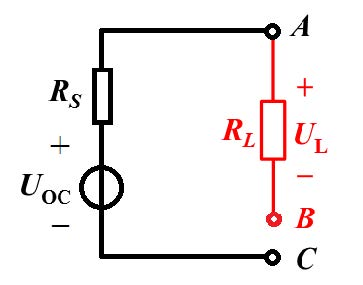
\includegraphics[width=0.5\linewidth]{FunR.jpg}}
\caption{函数信号发生器等效图}
\label{fig:FunR}
\end{figure}
\subsection{直流稳压电源(DC REGULATED POWER SUPPLY)}
直流稳压电源能够为的电子设备提供持续、稳定、满足负载要求的直流电能。本次实验使用的直流
稳压电源为GPD3303型,能够在0\~{}30V范围内连续可调,同时具有自动过载保护和短路保护功能。
\subsection{数字万用表(DIGITAL MULTMETER)}
数字万用表可以用来测量直流和交流电压以及电流、电阻、电容、二极管正向电压等,具有LCD显示器,最大
显示值为"19999",过量程显示"OPEN"。本次实验使用的是34450A型数字毫伏表。其注意事项如下:
\begin{itemize}
  \item 测量电阻时,被测量电阻不能带电。
  \item 测量电容时,要先放电,然后进行测量。
  \item 用数字万用表测正弦交流电压时,频率范围是40\~{}10kHZ。
\end{itemize}
\section{实验内容与步骤}
\subsection{实验内容}
	blablabla
\subsection{实验步骤}
	blablabla

\section{实验数据处理与分析}
\subsection{实验内容1}
	blablabla
\subsection{误差分析1}
	blablabla

\section{实验总结}
blablabla
\section{实验思考题}

\subsection{问题一}
总结各种仪器的使用方法以及注意事项。
\subsubsection{直流稳压电源}
基本使用方法如下:
\begin{enumerate}
  \item 正确连线后打开电源。输出电压的范围为0~30V,输出电流为0~3A。
  \item 选择工作模式和输出端,操作模式有独立/串联/并联三种。输出端有CH1/2/3。
  \item Voltage旋钮可以调节电压大小,Current旋钮可以调节电流大小,按下均可细调。
  \item 调节完成后,按下output旋钮进行输出。
  \item 当电流值小于输出设定值时,其工作在恒压源模式,CV亮绿灯。当电流达到输出设定值时,其工作咋恒流模式,CC亮绿灯。
  \item 通过跟踪开关可以选择电源的跟踪模式为串联或者并联,其可完成自动连线,可用于需要增强输出电压或者增强输出电流由或是需要两个电源电压/电流相等下工作的情形。
\end{enumerate}

注意事项如下:
\begin{enumerate}
  \item 预先设置合适的电压和电源值;
  \item "+","-"端口输出线不能短路;
  \item 与被测电路连接时,"+"、"-"输出线不能接错;
  \item 与被测电路连接时,一般先接与地线相连的端口。
\end{enumerate}
\subsubsection{函数信号发生器}
基本使用方法如下:
\begin{enumerate}
  \item 正确连线后打开电源。交流信号源可以用于产生多种交流输出波形,为被测电路提供信号。
  \item 选择合适的工作功能和输出端,选择需要的波形并调节参数,其输出频率范围不同波形不一致,一般为1μHz\~{}40MHz,对正弦波可达160MHz。
  \item 按下[Wave-forms]键即可调节波形,按下[parameter]键可以调节参数,参数可以通过大旋钮调节,也可以按下数字并选择单位进行调节。
  \item 输出负载可以选择高负载或者50Ω,按下[CH1/CH2]键,即可选择负载模式,一般采用高负载。
  \item 确定参数后,即可输出。
\end{enumerate}

注意事项如下:
\begin{enumerate}
  \item 输出线的两个夹子不能短路;
  \item 不能直接接到带有较高电流电压的两点之间;
  \item 与被测电路连接时,红夹子接信号源,黑夹子接地。
\end{enumerate}
\subsubsection{示波器}
基本使用方法如下:
\begin{enumerate}
  \item 正确连线后打开电源,选择需要的工作通道和模式。该款示波器的带宽是100MHz。不具有特殊部件下,输入模拟信号最大允许电压为300 Vrms,400 Vpk, 瞬间过电压 1.6kVpk。
  \item 首先调节波形稳定,首先粗调水平扫描速率至能比较好地看到波形,然后调节[Trigger]选择合适的源,可调节[Trigger]至稳定为止。
  \item 选择合适的耦合,按下通道后菜单即可选择,希望观测AC分量时选择AC耦合,希望观察DC分量时选择DC耦合。
  \item 选择正确的时间模式。“正常时间模式”显示的是一维的X(t)图形,X为信号。“X-Y”模式时显示的是XY空间的相图,意即两个信号分别作为X或Y分量。
  \item 调节水平扫描速率旋钮可以调整显示波形的周期数。
  \item 调节垂直灵敏度旋钮可以改变显示波形的高度,调节位移旋钮可以调整波形垂直位置。
  \item 进行测量时,按下[Cursors]按钮可以选择与移动光标进行测量。按下[Meas]可以自动测量和添加测量量。进行手动测量可以测量得到自动测量中没有预设的测量量,同时也可以认为减少噪声的干扰,进行更精确的测量。
\end{enumerate}

注意事项如下:
\begin{enumerate}
  \item 显示亮度应该合适,不能长时间固定亮点;
  \item 被测电压幅值不应该超过示波器最大允许输入电压;
  \item 被测电压频率不应超过其带宽值;
  \item 与被测电路连接时,探针接信号端,黑夹子接地;
  \item 读测波形参数时,波形高度应该超过屏幕高度的一半。
\end{enumerate}

\subsubsection{数字万用表}
基本使用方法如下:
\begin{enumerate}
  \item 正确连线,打开电源。
  \item 选择合适的工作模式,即选择需要测量的量。
  \item 调整合适的测量速度,量程由万用表自动选择。
\end{enumerate}

注意事项如下:
\begin{enumerate}
  \item 测量电阻时,被测电阻不能带电;
  \item 测量电容时,先放电后测量;
  \item 被测电压值不能超过端口允许值(直流1000VDC,交流750Vrms);
  \item 被测交流电压频率不应超过其带宽值(技术文档上写为100kHz,但实际10kHz已不准);
  \item 测试前,选择正确的端口接入测试引线,选择正确的功能键,选择合适的分辨率/速度;
  \item 表笔接在“mA”或“A”端口时,不能测电压(烧保险丝)。
\end{enumerate}
\subsection{问题二}
写出所有你能想到的函数信号发生器内阻的测量方法,并详细说明设计思路。
\subsubsection{方法一}
通过接一负载,在已知$U_oc$下可以一次测量得到电压,如前实验原理所说。若不知道$U_oc$,则可以通过连接如图 \ref{fig:FunR2}所示的电路,
测量出不同的U-I值,画出U-I曲线图。根据式 \ref{eqa:Rs2},通过拟合出斜率与截距,即可测量出内阻
\begin{equation}
U_l=U_{oc}-R_sI_l
\label{eqa:Rs2}
\end{equation}
  
\begin{figure}[htbp]
\centering
\fbox{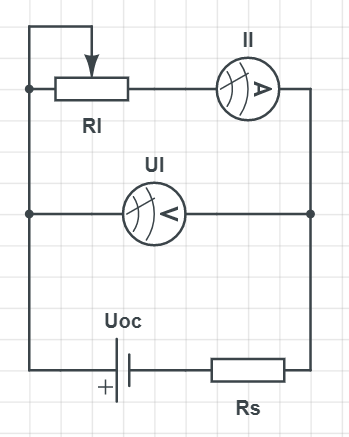
\includegraphics[width=0.2\linewidth]{FunR2}}
\caption{U-I法函数信号发生器内阻测量图}
\label{fig:FunR2}
\end{figure}

\subsection{方法二}
通过电阻箱与电压表测量,如图 \ref{fig:FunR3}所示。调节电阻箱的值为$R_{l1}$与$R_{l2}$分别测量。
根据公式 \ref{eqa:Rs},得到两组式子,联立消去$U_oc$即可解出$R_s$的值。
\begin{figure}[htbp]
  \centering
  \fbox{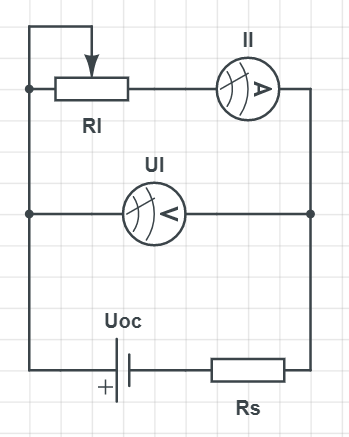
\includegraphics[width=0.2\linewidth]{FunR2}}
  \caption{电阻箱电压表函数信号发生器内阻测量图}
  \label{fig:FunR3}
  \end{figure}
  
\subsection{方法三}
通过电阻箱与电流表测量,如图 \ref{fig:FunR4}所示。调节电阻箱的值为$R_{l1}$与$R_{l2}$分别测量。
根据公式 \ref{eqa:Rs3},得到两组式子,联立消去$U_oc$即可解出$R_s$的值。
\begin{equation}
  I\left(R_s+R_l\right)=U_{oc}
\label{eqa:Rs3}
\end{equation}
    
\begin{figure}[htbp]
  \centering
  \fbox{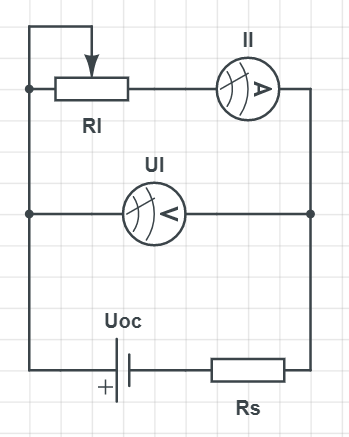
\includegraphics[width=0.2\linewidth]{FunR2}}
  \caption{电阻箱电流表法函数信号发生器内阻测量图}
  \label{fig:FunR4}
  \end{figure}
  
\end{document}
